% main.tex

\documentclass[lang=cn,10pt,newtx,thmcnt=section,chinesefont=founder]{vividbook}
% mode = fancy

% header.tex

% for LinearAlgebra_ECNU

\setcounter{tocdepth}{3}


% 调试用
% \usepackage{zhlipsum}
% \usepackage{syntonly}
% \syntaxonly

% 本文档命令
\usepackage{array}
\usepackage{float}
\usepackage{subfig,caption}

\usepackage{bm}

%NiceMatrix
\usepackage{nicematrix}
\NiceMatrixOptions{cell-space-limits = 1.5pt}
\usepackage{arydshln}

\newcommand{\ccr}[1]{\makecell{{\color{#1}\rule{1cm}{1cm}}}}

% 修改标题页的橙色带
\definecolor{customcolor}{RGB}{245, 250, 246}
\colorlet{coverlinecolor}{customcolor}


\definecolor{framegolden}{RGB}{0, 174, 247} % 控制外框颜色


%%% Local Variables:
%%% mode: LaTeX
%%% TeX-master: "./main.tex"
%%% coding: utf-8
%%% End:


\title{线性代数笔记:基于ECNU讲义}
\subtitle{满coop会长再也不用在考前组织学习会}

\author{吃盐水棒冰活下去!}
\date{\today}
\version{V0}

\logo{YamadaRyo1.png}
\cover{frontcover.png}

\extrainfo{“你指尖跃动的电光,是我此生不灭的信仰,唯我超电磁炮永世长存!”\\{\footnotesize “君の指先を舞ってる電光は、私の一生変わらない信仰であり、このレールガンだけが永遠に生きてる!”}}

\addbibresource[location=local]{reference.bib} % 参考文献

\begin{document}
\chapterimage{FutabaRio.png}
\maketitle
\frontmatter
\tableofcontents
\mainmatter
% chapters/cha1.tex

\chapterimage{RainyAnnSubway.png}

\chapter{基础知识}
\label{chap:cha1}
\begin{center}
    八月已经这么热了,那十二月岂不是会热成炼狱吗?
\end{center}
\rightline{—— 坂本 龙司}
\vspace{-5pt}
\begin{center}
    \pgfornament[width=0.36\linewidth,color=lsp]{88}
\end{center}
\section{线性方程组与矩阵消元法}
\label{sec:11}

我们需要回顾中学中学过的二元一次和三元一次方程组的求解问题,引出对一般的线性方程组的理解。在这里,将通过中学的解析几何和向量知识对线性方程组有更深的理解。

\subsection{二元一次方程组}
\label{sec:111}

对于一元一次方程组\(ax = b \),初中数学告诉我们,有三种情况。
\begin{enumerate}
\item[唯一解] 当\(a \neq 0 \)时,方程有唯一解\(x = \frac{b}{a} \)
\item[无解] 当\(a=0 \)且\(b \neq 0\)时,方程无解
\item[无穷多解] 当$a=0$且$b \neq 0$时,方程有无穷多解,$x$为任意常数
\end{enumerate}

现在,考虑未知量为\(x_{1},x_{2} \)的二元一次方程的求解问题。\[
  \begin{cases}
    a_{11} x_{1} + a_{12} x_{2} &= b_{1} \\
    a_{21} x_{1} + a_{22} x_{2} &= b_{2} \\
  \end{cases}
\]

\subsubsection{有唯一解的情况}
\label{sec:1111}

% 例1.1.1
\begin{example}
  求解二元一次方程组\[
    \begin{cases}
      x_{1} + x_{2} &= 1,\\
      x_{1} - x_{2} &= 3. \\
    \end{cases}
    \]
  \end{example}
  \begin{solution}
    通过消元法,有
    \begin{align}
    &  \begin{cases}
        x_{1} + x_{2} &= 1,\\
        x_{1} - x_{2} &= 3. \\
    \end{cases}
      \label{equationset:1111a} \\
      \longrightarrow
     &  \begin{cases}
        x_{1} + x_{2} &= 1,\\
        -2x_{2} &= 2.\\
      \end{cases}
      \label{equationset:1111b}
      \\
      \longrightarrow
   &    \begin{cases}
        x_{1} + x_{2} &=1,\\
        x_{2} &= -1.\\
      \end{cases} \notag \\
      \longrightarrow
    &   \begin{cases}
        x_{1} &= 2,\\
        x_{2} &= -1.\\
      \end{cases} \label{equationset:1111solution} 
    \end{align}
  \end{solution}
  \begin{solution}
    接下来,再从行图像的观点查看此方程组。解析几何知道,方程组的每一行可以表示为平面直角坐标系中的一条直线。如图~\ref{fig:1111rows}所示,原问题即求解两直线交点的坐标。而每一次消元则变成了绕交点对直线进行旋转的过程。

    \begin{figure}[H]
      \centering
      \subfloat[对应于~\ref{equationset:1111a}]{% *-* coding: utf-8 *-*
% 1.1.1 row picture a

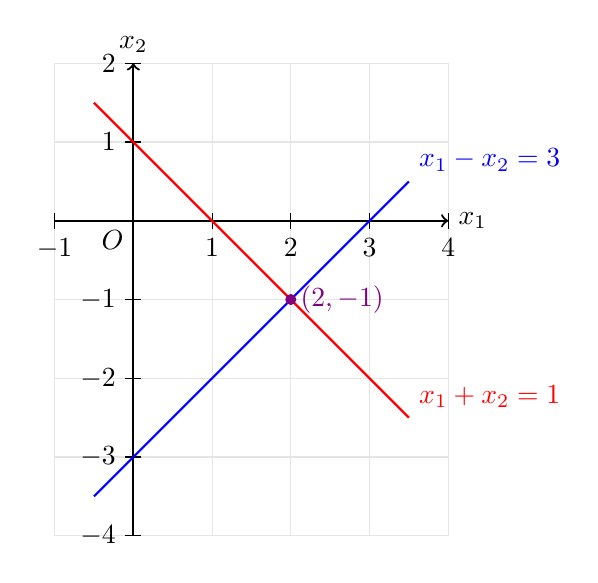
\begin{tikzpicture}[scale=1]

   % 绘制网格
    \draw[gray!20] (-1,-4) grid (4,2);
   
    % 绘制坐标轴
    \draw[->, thick] (-1,0) -- (4,0) node[right] {$x_{1}$};
    \draw[->, thick] (0,-4) -- (0,2) node[above] {$x_{2}$};
    
    
    % 标记坐标轴刻度
    \foreach \x in {-1,1,2,3,4}
        \draw (\x,0.1) -- (\x,-0.1) node[below] {$\x$};
    \foreach \y in {-4,-3,-2,-1,1,2}
        \draw (0.1,\y) -- (-0.1,\y) node[left] {$\y$};
    
    % 绘制直线 x+y=1 (红色)
    \draw[red, thick, domain=-0.5:3.5] plot (\x, {1-\x}) node[above right] {$x_{1}+x_{2}=1$};
    
    % 绘制直线 x-y=3 (蓝色)
    \draw[blue, thick, domain=-0.5:3.5] plot (\x, {\x-3}) node[above right] {$x_{1}-x_{2}=3$};
    
    % 计算并标记交点 (2,-1)
    \coordinate (A) at (2,-1);
    \fill[violet] (A) circle (2pt);
    \node[right, violet] at (A) {$(2,-1)$};
    
    % 标记原点
    \node[below left] at (0,0) {$O$};
\end{tikzpicture}
}
      \hspace{1cm}
      \subfloat[对应于~\ref{equationset:1111b}]{\input{tikzs/111Rowb.tikz}}
      \\
      \subfloat[对应于~\ref{equationset:1111solution}]{\input{tikzs/111Rowc.tikz}}
      \caption{用行图像解方程}
      \label{fig:1111rows}
    \end{figure}
    \end{solution}
    
\subsection*{三元一次方程组}
\label{secex:ThreeUnknownsEquations}


\subsection{线性方程组的矩阵消元法}
\label{sec:112}

将上述对方程组的讨论推广至更加一般的情形:有n个未知数和m个方程的线性方程组\eqref{eq:EquationsSetNormal}。
\begin{equation}
  \label{eq:EquationsSetNormal}
  \begin{cases}
    a_{11}x_{1} + a_{12}x_{2} +  \ldots &= \quad b_{1} \\
    a_{21}x_{1} + a_{22}x_{2} +  \ldots &= \quad b_{2} \\
                                        &\vdots  \\
    a_{m1}x_{1} + a_{m2}x_{2} +  \ldots &= \quad b_{m} \\
  \end{cases}
\end{equation}
其中$a_{ij}$和$b_{i}$是系数常数,$x_{i}$是未知元。

为了解出这个线性方程组,我们所需要的“信息”显然只有这些系数,诸如加号等号这些记号,都不是非常必要的。我们可以用矩阵记载这些系数的信息,接下来先引入矩阵的定义。

%定义1.1.4
\begin{definition}{矩阵}
  \label{def:Matrix}
  一个$m \times n$的\textbf{矩阵}是一个有m行和n列元素的巨型阵列,矩阵中的元素可以使数字、符号,甚至可以是函数。% \footnote{用粗斜体表示,其实是用\verb|\bm|命令打出的记号}
  
  例如,我们可以将一个$m \times n$的矩阵记作
  \begin{equation}
    \label{matrix:NormalMatrix}
\bm{A} = (a_{ij})_{m \times n} 
\begin{pmatrix}
  a_{11} & a_{12} & \ldots & a_{1j} & \ldots & a_{1n} \\
  a_{21} & a_{22} & \ldots & a_{2j} & \ldots & a_{2n} \\
  \vdots & \vdots &       & \vdots &        & \vdots \\
  a_{i1} & a_{i2} & \ldots & a_{ij} & \ldots & a_{in} \\
  \vdots & \vdots &       & \vdots &        & \vdots \\
  a_{m1} & a_{m2} & \ldots & a_{mj} & \ldots & a_{mn} \\
\end{pmatrix} 
\end{equation}
其中,位于的$i$行和第$j$列的元素$a_{ij}$成为$\bm{A}$的$(i,j)$元素,而$i$和$j$分别称为$a_{ij}$的行标和列标。
\end{definition}


显然地,每个方程组的“系数信息”都可以抽象地排列成为与之对应的矩阵。如果只记载排列未知数的系数信息,则为系数矩阵;如果同时还记载排列了等号右侧的常数,则为增广矩阵。

\begin{definition}{系数矩阵与增广矩阵}
  \label{def:CoefficientAugmentedMatrix}
  对于线性方程组\eqref{eq:EquationsSetNormal}而言,其常数可以构成系数矩阵\(\bm{A} \)和增广矩阵$\bm{A}'$.
  \begin{equation}
    \label{matrix:CoefficientAugmentedMatrix}
    \bm{A} =
    \begin{pmatrix}
      a_{11} & a_{12} & \cdots & a_{1n} \\
      a_{21} & a_{22} & \cdots & a_{2n} \\
      \vdots & \vdots &     & \vdots \\
      a_{m1} & a_{m2} & \cdots & a_{mn} \\
    \end{pmatrix} \quad
    \bm{A}' =
    \left(
      \begin{array}{cccc:c}
        a_{11}&a_{12}&\cdots&a_{1n}&b_{1} \\
        a_{21}&a_{22}&\cdots&a_{2n}&b_{2} \\
        \vdots&\vdots& &\vdots&\vdots \\
        a_{m1}& a_{m2}& \cdots& a_{mn}&b_{m} \\
      \end{array}
    \right)
  \end{equation}
  
\end{definition}

\begin{definition}{矩阵的初等变换}
  \label{def:ElementaryTransformationsOfMatrix}
  
  矩阵的\textbf{初等行(列)变换},又合称\textbf{初等变换},有以下三种:
  \begin{enumerate}
  \item \textbf{对换行(列)变换}:互换两行(列)
  \item \textbf{倍乘行(列)变换}:某行(列)乘以一个非零常数$k$
  \item \textbf{倍加行(列)变换}:某行(列)乘以一个常数$k$(允许为零,即不变换)后,加至另一行(列)
  \end{enumerate}
\end{definition}


所以,通过对系数矩阵做初等变换可以依次得到行阶梯形和行简化阶梯形,用明文给出其定义\cite{LinearAlgebraAndItsApplications}。

\begin{definition}{行阶梯形}
  \label{def:RowEchelonForm}
  一个矩阵被称为\textbf{行阶梯形}(或\textbf{阶梯形}),它需要具有以下三个性质。

  我们称每一行中最左边的非零元素为“先导元素”。
  \begin{enumerate}
  \item 每一非零行都在每一零行之上(所有非零行全在矩阵最后)
  \item 每一行的先导元素所在的列都位于其上一行(若有)的右边
  \item 任意先导元素所在列下方元素(若有)均为零
  \end{enumerate}

  这样的矩阵会有以下形式:
  \begin{equation}
    \label{matrix:RowEchelonForm}
      \left(
        \begin{array}{*{13}{c}:c}
          \bullet & \ast & \cdots & \ast & \ast & \cdots & \ast & \ast & \cdots & \ast & \ast & \cdots & \ast & \ast \\
                  &      &    & \bullet  & \ast & \cdots & \ast & \ast & \cdots & \ast & \ast & \cdots & \ast & \ast \\
                  &      &        &      &      &    & \bullet  & \ast & \cdots & \ast & \ast & \cdots & \ast & \ast \\
                  &      &        &      &      &        &      &      & \ddots & \vdots & \vdots & & \vdots  & \vdots \\
                  &      &        &      &      &        &      &      &     & \bullet & \ast & \cdots & \ast & \ast \\
                  &      &        &      &      &        &      &      &     &         &      &        &      &      \\
          
      \end{array}
    \right)
  \end{equation}
  其中,$\bullet$标记一定不为零的元素,他们即是每一行的“先导元素”。$\ast$标记可能不为零的元素,其余位置全为零元素。

  在虚线左侧的列中,$\bullet$所在的列称为\textbf{主列},对应的未知元称为\textbf{主元},其余列称为\textbf{自由列},对应的未知元称为\textbf{自由元}。同时,阶梯形中至少有一个元素不为零的行称为\textbf{非零行},全部元素都为零的行称为\textbf{零行},而非零行的个数则称为该阶梯形的\textbf{阶梯数}。
\end{definition}

由于行阶梯形是通过矩阵初等变换得到的,相当于对方程组进行了消元的操作,因此它所代表的线性方程组所对应的解和原方程组相同。
\begin{conclusion}
  若记系数矩阵对应的行阶梯形(虚线左侧的部分)的阶梯数$r$,增广矩阵(含虚线右侧的整体)对应行阶梯形的阶梯数$r'$,可以得到$r$、$r'$,以及方程个数$m$和未知元个数$n$之间满足的关系:
  \begin{enumerate}
  \item \( \mathbf{0 \leq r' - r \leq 1} \) 由于增广矩阵对应的阶梯形和系数矩阵对应的阶梯形左侧都是一致的,只有最左侧多出来一列。如果这一列末尾有一个单独的非零常数(不可能超过一个,否则不符合行阶梯形“每行先导元素下方全是零”的要求),则$r' - r = 1$;反之,则两矩阵的主列都在虚线左侧,数目相等。
  \item \(\mathbf{0 \leq r \leq min \left\{ m,n \right\} } \) 对于一个阶梯形,其最极限的情况,显然是从左上角第一个元素作为先导元素开始,其右下方的元素也是线性元素,直至矩阵的边界,也就是\(min \left\{ m,n \right\} \)个
  \item \(\mathbf{0 \leq r' \leq min \left\{ m,n+1 \right\} } \)同上。
  \end{enumerate}
\end{conclusion}
\begin{definition}{行简化阶梯形}
  \label{def:rref}
  如果一个\textbf{行阶梯形}还具有以下性质,则称之为\textbf{行简化阶梯形}(或\textbf{简化阶梯形})。
  \begin{enumerate}
  \item 每一非零行的先导元素是1
  \item 每一先导元素1是该元素所在列唯一的非零元素(即每个先导元素上方的元素也全部是零)
  \end{enumerate}
    这样的矩阵会有以下形式:
    \begin{equation}
      \label{matrix:rref}
      \left(
        \begin{array}{*{13}{c}:c}
             1    & \ast & \cdots & 0    & \ast & \cdots &  0   & \ast & \cdots &  0   & \ast & \cdots & \ast & \ast \\
                  &      &    &    1     & \ast & \cdots &  0   & \ast & \cdots &  0   & \ast & \cdots & \ast & \ast \\
                  &      &        &      &      &    &    1     & \ast & \cdots &  0   & \ast & \cdots & \ast & \ast \\
                  &      &        &      &      &        &      &      & \ddots & \vdots & \vdots & & \vdots  & \vdots \\
                  &      &        &      &      &        &      &      &     &    1    & \ast & \cdots & \ast & \ast \\
                  &      &        &      &      &        &      &      &     &         &      &        &      &      \\
          
      \end{array}
    \right)
\end{equation}
    可以发现,每个\textbf{简化行阶梯形}与对应的\textbf{行阶梯形},其主元列和自由列有完全相同的位置,且两者有相同的阶梯数。
  \end{definition}
\begin{remark}
  一个矩阵对应的行阶梯形在一般情况下并不唯一(在用Gauss消元法完成后,用Jordan消元法回代过程中产生的每一个矩阵显然都是行阶梯形。)但其对应的行简化阶梯形是唯一的。%need to complete ref
\end{remark}

% 定理1.1.7
\begin{theorem}{线性方程组解的判别定理}
  \label{thm:DeterminationThmForSolutionsOfLinearSystemsOfEquations}
  考虑线性方程组\eqref{eq:EquationsSetNormal},并设其对应的\textbf{系数矩阵}和\textbf{增广矩阵}\eqref{matrix:CoefficientAugmentedMatrix}相应的行阶梯形中的\textbf{阶梯数}分别为$r$和$r'$,则有以下结论:
  \begin{enumerate}
  \item 若\(r<r' \),则方程组无解。\textit{方程组约束太多,没有符合条件的数组。}
  \item 若\(r = r' = n\),则方程组有唯一解。\textit{方程组约束不多不少,有唯一的数组符合等式约束条件。}
  \item 若\(r = r' < n\),则方程组有无穷多解。\textit{方程组约束不够,有很多数组符合等式。}
  \end{enumerate}
\end{theorem}


\subsection{齐次与非齐次线性方程组}
\label{sec:113}
接下来,我们来讨论线性方程组解的情况。为了便于讨论,先给它们下一番定义。

\begin{definition*}
  对于线性方程组\eqref{eq:EquationsSetNormal},形如\(x_{1} = x_{2} = \cdots = x_{n} = 0 \)的解称为\textbf{零解};至少存在一个$x_{i} \neq 0$的解称为\textbf{非零解}。

  当方程组有无穷多解时,其一般形式的解称之为\textbf{通解}或\textbf{一般解}。

  一组可使该线性方程组成立的\(x_{1},x_{2},\cdots,x_{n} \)称之为此线性方程组的\textbf{特解}。
\end{definition*}

\begin{remark}
  在这里,向量的概念尚未引入,因而我们认为线性方程组的\textbf{解}只是一组等式的形式。可以把每个未知数对应的值排成一列,就可以得到一个\textbf{向量},该向量维数等于未知数个数,每个方向的分量是每个未知数对应的值,我们也可以认为这个\textbf{向量}是这个方程组的\textbf{解},因为它记载了方程组解的信息。
\end{remark}


分析方程式等式右侧常系数的情况,显然全部为0是一种特殊的,易于讨论的情况,可以下面多个角度认识到这一点:
\begin{enumerate}
\item 在对矩阵用Gauss-Jordan消元法时,不需要变动右侧的系数
\item 只需要系数矩阵就可以得到这个方程组的全部信息(当然,“这个方程组右侧常系数全部都是0”也是一个信息,但显然是更方便于获悉一个更复杂的增广矩阵)
\item 每列的图像都经过原点
\item 列图像的线性组合最后会经过原点
\end{enumerate}

\vspace{1cm}
这种特殊的情况,我们称之为“\textbf{齐次线性方程组}”。

\begin{definition}{齐次线性方程组}
  \label{def:HomogeneousLinearEquations}
  如果方程组中等号右侧的项\(b_{1},b_{2},\cdots,b_{m} \)均为零,即具有以下形式,则称为“齐次线性方程组”。
  \begin{equation}
    \begin{cases}
      \label{eq:HomogenenousLinearEquations}
    a_{11}x_{1} + a_{12}x_{2} +  \ldots &= \quad 0 \\
    a_{21}x_{1} + a_{22}x_{2} +  \ldots &= \quad 0 \\
                                        &\vdots  \\
    a_{m1}x_{1} + a_{m2}x_{2} +  \ldots &= \quad 0 \\
  \end{cases}
\end{equation}
\end{definition}

“方程组右侧常数全部都是零”的否命题为“方程式右侧常数存在至少一个不是零”,因而可以给出“非齐次线性方程组”的定义。
\begin{definition}{非齐次线性方程组}
  \label{def:NonHomogeneousLinearEquations}
  若方程组具有以下形式,且等号右侧的项不全为零,即\(\exists i , b_{i} \neq 0 \),则称该方程组为“\textbf{非齐次线性方程组}”,而$b_{1},b_{2},\cdots,b_{n}$称为\textbf{非齐次项}。
  \begin{equation}
    \begin{cases}
            \label{eq:NonHomogenenousLinearEquations}
    a_{11}x_{1} + a_{12}x_{2} +  \ldots &= \quad b_{1} \\
    a_{21}x_{1} + a_{22}x_{2} +  \ldots &= \quad b_{2} \\
                                        &\vdots  \\
    a_{m1}x_{1} + a_{m2}x_{2} +  \ldots &= \quad b_{m} \\
  \end{cases}
\end{equation}

同时,我们又称齐次线性方程组\eqref{eq:HomogenenousLinearEquations}是非齐次线性方程组\eqref{eq:NonHomogenenousLinearEquations}的\textbf{导出组}。
\end{definition}
\begin{remark}
  代入可以知道,\textbf{齐次线性方程组}必有\textbf{零解},而\textbf{非齐次线性方程组}必没有\textbf{零解}。
\end{remark}

由于齐次线性方程组必有零解,它不可能无解。我们可以将定理~\ref{thm:DeterminationThmForSolutionsOfLinearSystemsOfEquations}限定在齐次线性方程组的范围之内,得到以下定理:

% 定理1.1.10
\begin{theorem}{齐次线性方程组解的判别定理}
  \label{thm:DeterminationThmForSolutionsOfHomogeneousLinearSystemsOfEquations}
  设齐次线性方程组\eqref{eq:HomogenenousLinearEquations}的系数矩阵$\bm{A}$中对应的行阶梯形中非零行的个数为$r$。
  \begin{enumerate}
  \item 若$r = n$,约束充足,该方程组只有零解
  \item 若$r < n$,约束不足,该方程组有非零解
  \end{enumerate}
\end{theorem}

% 命题1.1.13
\begin{proposition}{齐次线性方程组存在非零解的充分条件}
  \label{pro:11thirteen} %这个用英语驼峰命名真的有点过于逆天了
  设齐次线性方程组对应的系数矩阵为$m \times n$阶矩阵$\bm{A}$。若$m<n$,则该方程组必有非零解。
\end{proposition}
\begin{proof}
  由于$\bm{A}$为$m \times n$阶矩阵,可知$\mathrm{rref} \bm{A}$也是$m \times n$阶矩阵。注意到$m<n$,自然有$\mathrm{rref} \bm{A}$中非零行个数$r$满足$r \leq m < n$,由定理~\ref{thm:DeterminationThmForSolutionsOfHomogeneousLinearSystemsOfEquations}第二种情况知:相应的齐次线性方程组必有零解。
\end{proof}


\section{向量空间与相关性}
\label{sec:12}

\subsection{平面向量}
\label{sec:121}

暂时跳过,需要tikz绘图,之后再补。% need to be completed!

\begin{definition*}{平面向量的加法和数乘}
  现有任意两个平面向量\(\bm{\alpha} = (a_{1},a_{2}),\bm{\beta}=(b_{1},b_{2}) \),又有任意实数$k$。

 平面向量的加法和数乘分别定义为
 \begin{equation}
   \label{eq:AdditionAndScalarMultiplicationOfPlaneVectors}
   \bm{\alpha} + \bm{\beta} = (a_{1}+b_{1} , a_{2}+b_{2} ) \qquad k \bm{\alpha} = (k a_{1},k a_{2})
 \end{equation}
 画图介绍平面向量的共线问题。

\end{definition*}
 \begin{proposition}{平面向量的充分必要条件}
   \label{pro:PlaneVectorCollinear}
 \end{proposition}

\subsection{m维向量与向量空间\texorpdfstring{$\mathbb{R}^m$}{}}
\label{sec:122}

从平面向量的坐标表示出发,拓宽到三维空间,以及更加高维的m维空间,引入m维向量的概念。

% 定义1.2.1
\begin{definition}{m维向量}
  \label{def:MDimensionalVector}
  我们称$m \times 1$和$1 \times m$的矩阵分别为m维\textbf{列向量}与m维\textbf{行向量}。使用记号\[
\bm{\alpha} =
\begin{pmatrix}
  a_{1} \\ a_{2} \\ \vdots \\ a_{m} \\
\end{pmatrix}
\quad \text{与} \quad
\bm{\alpha}^{\mathrm{T}} = (a_{1},a_{2},\cdots,a_{m})
\]  分别表示m维\textbf{列向量}与m维\textbf{行向量}。其中,列向量的上角标$T$代表转置运算,即把向量$\bm{\alpha}$翻转成行的形式。
\end{definition}

在有了m维向量的概念后,引入实向量和实向量空间的概念。

% 定义1.2.2
\begin{definition}{实向量和实向量空间$\mathbb{R}^{m}$}
  \label{def:RealVectorSpace}
  若对\(\forall i = 1,2,\cdots,m \),定义~\ref{def:MDimensionalVector}中的$a_{i}$满足\(a_{i} \in \mathbb{R} \),我们称相应的$\bm{\alpha}$或$\bm{\alpha}_{T}$为\textbf{m维实向量}。

  全体m维列(或行)实向量所组成的集合为m维\textbf{实向量空间},记作$\mathbb{R}^{m}$。
\end{definition}

但为了进行下面对m维向量加法和乘法的讨论,先需要定义一个特别的m维向量:\textbf{零向量},以及一个与$\bm{\alpha}$相关的向量:\textbf{负向量}。
\begin{definition}{零向量和负向量}
  \label{def:ZeroVectorAndNegativeVector}
  规定m维\textbf{零(列)向量}\[
    \bm{0} = (0,0,\cdots,0)^{\mathrm{T}}
  \]
  与$\bm{\alpha}$的负向量\[
    - \bm{\alpha} = (-a_{1},-a_{2},\cdots,-a_{m})^{\mathrm{T}}。
    \]
  \end{definition}

仿照平面向量的相关定义,即\eqref{eq:AdditionAndScalarMultiplicationOfPlaneVectors},可以引入m维向量加法和数乘的定义,并得到有关于其加法和乘法的一些事实。

\begin{definition}{m维向量的加法}
  \label{def:AdditionOfMDimensionalVectors}
  设有两个m维实向量:\[
\bm{\alpha}=(a_{1},a_{2},\cdots,a_{m})^{\mathrm{T}},\bm{\beta}=(b_{1},b_{2},\cdots,b_{m})^{\mathrm{T}}
\]
现定义$\bm{\alpha}$和$\bm{\beta}$的加法\[
\bm{\alpha} + \bm{\beta} = (a_{1}+b_{1} , a_{2}+b_{2}, \cdots ,a_{m}+b_{m})^{\mathrm{T}}
  \]
\end{definition}

\begin{axiom}{加法公理}
  \label{axi:VectorsAddition}
  \( \forall \bm{\alpha},\bm{\beta},\bm{\gamma} \in \mathbb{R}^{m}\),有以下四条性质成立(可以很方便的用向量加法的定义验证):
  \begin{enumerate}
  \item \textbf{加法交换律} \quad  \(\bm{\alpha}+\bm{\beta} = \bm{\beta} + \bm{\alpha}\)
  \item \textbf{加法结合律} \quad  \( ( \bm{\alpha}+\bm{\beta} ) +\bm{\gamma} = \bm{\alpha} + (\bm{\beta} + \bm{\gamma}) \)
  \item \textbf{零向量存在性} \quad 存在零向量$\bm{0}$,使得\(\bm{\alpha} + \bm{0} = \bm{\alpha} \)
  \item \textbf{负向量存在性} \quad 存在负向量$- \bm{\alpha}$,使得\(\bm{\alpha} + ( - \bm{\alpha}) = 0 \)
  \end{enumerate}
\end{axiom}

\begin{definition}{m维向量的数乘}
  \label{def:ScrlarMultiplicationOfMDimensioalVectors}
  设有任意实常数k以及m维实向量\(\bm{\alpha}=(a_{1},a_{2},\cdots,a_{m})^{\mathrm{T}}\),其数乘为:\[
k \bm{\alpha} = (k a_{1}, k a_{2}, \cdots , k a_{m} )^{\mathrm{T}}
    \]
  \end{definition}

  \begin{axiom}{数乘公理} \label{axi:VectorScalarMultiplication}
      \( \forall \bm{\alpha},\bm{\beta} \in \mathbb{R}^{m} , \forall k,l \in \mathbb{R}\),有以下四条性质成立(可以很方便的用向量数乘的定义验证):
    \begin{enumerate}
    \item \textbf{单位数} \(1 \bm{\alpha} = \bm{\alpha} \)
    \item \textbf{数乘结合律} \(k (l \bm{\alpha}) = (kl) \bm{\alpha} \)
    \item \textbf{数乘对数的分配律} \((k+l) \bm{\alpha} = k\bm{\alpha}+l\bm{\alpha} \)
    \item \textbf{数乘对向量的分配律} \(k(\bm{\alpha} + \bm{\beta}) = k \bm{\alpha} + k \bm{\beta} \)
    \end{enumerate}
  \end{axiom}
  \begin{remark}
    我们可以很方便的利用给出的加法定义~\ref{def:AdditionOfMDimensionalVectors}和数乘定义~\ref{def:ScrlarMultiplicationOfMDimensioalVectors},验证这些所谓的公理~\ref{axi:VectorsAddition}和~\ref{axi:VectorScalarMultiplication}。但事实上,这种验证之所以可以成立,完全依赖于我们所给出的良好定义。从抽象数学的观点来看,这些公理本身的成立才是保证代数运算的关键。也就是说,只要运算满足这些性质,就可以在代数意义上被我们称为“加法”和“数乘”。另一方面,我们注意到上述两个定义都是基于坐标的,但向量的加法和数乘只要在抽象的向量空间$\mathbb{R}^{m}$中就可以进行,坐标并不是十分必要的。所以,八条公理在逻辑上先于两条基于坐标运算的定义。
  \end{remark}

  基于这些结论,我们可以得出五条推论:
  % 推论1.2.4
  \begin{corollary}
    \label{cor:Vectors124}
    设$\bm{0}$是$\mathbb{R}^{m}$中的任意向量,$k$是任意常数,则有:
    \begin{enumerate}
    \item \(\bm{0} + \bm{\alpha} = \bm{\alpha},
(-\bm{\alpha}) + \bm{\alpha} = \bm{0}      \)
\item 零向量$\bm{0}$唯一,负向量$-\bm{\alpha}$唯一
\item \( 0 \bm{\alpha} = \bm{0}, (-1)\bm{\alpha} = 1\bm{\alpha}  \)
\item \(k \bm{0} = \bm{0} \)
\item 若$k \bm{\alpha} = 0$则有$k = 0$或$\bm{\alpha} = \bm{0}$
    \end{enumerate}
  \end{corollary}
  \begin{proof}
    need to be completed
  \end{proof}
\vspace{1cm}
现在,对于一个集合,我们对其中的元素进行“加法”和“数乘”运算。有时,我们希望运算的结果始终保持在集合之中,也就是说,我们希望集合中的元素对这些运算满足“\textbf{封闭性}”,对于由数字构成的集合,我们便可以引入\textbf{数域}的概念。

% 定义1.2.6
  \begin{definition}{数域}
    \label{def:NumberField}
    设$\mathbb{F}$是一个数集,若其满足:
    \begin{enumerate}
    \item 数\(0,1 \in \mathbb{F} \)
    \item $\mathbb{F}$关于数的四则运算封闭
    \end{enumerate}
    则称$\mathbb{F}$是一个\textbf{数域}。
  \end{definition}

  \begin{example}
    实数集$\mathbb{R}$,复数集$\mathbb{C}$,有理数集$\mathbb{Q}$都构成数域
  \end{example}
  \begin{example}
    自然数集$\mathbb{N}$,整数集$\mathbb{Z}$,和区间$[0,1]$都不是数域。
  \end{example}
  \begin{example}
    数集\( A = \left\{ a+b \sqrt{2} | a,b \in \mathbb{Q} \right\} \)是一个数域。
  \end{example}

  上述例子都可以通过定义直接证明或证伪。

  引入了数域的概念之后,我们可以类比m维实向量的相关讨论,将定义加以推广:
  \begin{definition*}{数域$\mathbb{F}$上的m维向量、向量空间$\mathbb{F}^{m}$}
    \textbf{数域$\mathbb{F}$上的m维向量}$\alpha$ \[ 
\bm{\alpha} = \left( a_{1},a_{2},\cdots,a_{m} \right)^{\mathrm{T}}, \quad a_{1},a_{2},\cdots,a_{m} \in \mathbb{F}
\]
而由这些向量的全体可以构成\textbf{数域$\mathbb{F}$上的向量空间$\mathbb{F}^{m}$}
  \end{definition*}

\subsection{线性相关性}
\label{sec:123}

我们在~\ref{sec:121}中讨论过两个向量共线的充分必要条件,即命题~\ref{pro:PlaneVectorCollinear},接下来我们将其在两个方面加以推广:
\begin{enumerate}
\item 向量维数从2到一般的正整数m,即从平面向量到高维向量
\item 向量个数从2到一般的正整数n
\end{enumerate}

对于命题~\ref{pro:PlaneVectorCollinear}右侧的表述,我们引入\textbf{线性组合}的概念,进而表述\textbf{线性相关}和\textbf{线性无关}的概念。

% 定义1.2.9
\begin{definition}{线性组合}
  \label{def:LinearCombination}
  设有\(\bm{\alpha}_{1},\bm{\alpha}_{2},\cdots,\bm{\alpha}_{n},\bm{\beta} \in \mathbb{R}^{m} \),若存在常数\(k_{1},k_{2},\cdots,k_{n} \)使得\[
\bm{\beta} = \sum_{j=1}^{n} \left( k_{j} \bm{\alpha}_{j} \right)
\] 则称向量$\bm{\beta}$是向量\(\bm{\alpha}_{1},\bm{\alpha}_{2},\cdots,\bm{\alpha}_{n} \)的\textbf{线性组合},或称向量$\bm{\beta}$可被\(\bm{\alpha}_{1},\bm{\alpha}_{2},\cdots,\bm{\alpha}_{n} \)\textbf{线性表示},常系数\(k_{1},k_{2},\cdots,k_{n} \)称为\textbf{组合系数}或者\textbf{表示系数}。
\end{definition}

% 定义1.2.10
\begin{definition}{线性相关}
  \label{def:LinearDependence}
  设有\(\bm{\alpha}_{1},\bm{\alpha}_{2},\cdots,\bm{\alpha}_{n} \in \mathbb{R}^{m} \),若存在\textbf{不全为零}的常数\(k_{1},k_{2},\cdots,k_{n} \),使得\[
\sum^{n}_{j=1} \left( k_{j} \bm{\alpha}_{j} \right) = 0
    \]则称\(\bm{\alpha}_{1},\bm{\alpha}_{2},\cdots,\bm{\alpha}_{n} \)\textbf{线性相关}。
  \end{definition}
  \begin{note}
    由于线性组合的系数是“任意常数”,那么实际上每个$\bm{\alpha}$的长度并不是十分重要的(只要其长度非0,可以通过乘常数伸展为任意的长度),唯一有用的信息是其方向。在没有零向量的情况下,若将每个$k_{j} \bm{\alpha}_{j}$视作位移,问题就变成了:从原点出发,能否依次按\(\bm{\alpha}_{1},\bm{\alpha}_{2},\cdots,\bm{\alpha}_{n}\)的方向移动数次,至少有一次离开原点(对应于“系数不全为零”),最后再回到原点?
  \end{note}

  将\textbf{线性相关}的定义~\ref{def:LinearDependence}用对偶法则加以修改,并注意到所有系数全为0时,\(\bm{\alpha}_{1},\bm{\alpha}_{2},\cdots,\bm{\alpha}_{n}\)的线性组合必为$\bm{0}$,可以得到\textbf{线性无关}的定义~\ref{def:LinearIndependence}。
  % 定义1.2.11
  \begin{definition}{线性无关}
    \label{def:LinearIndependence}
    设\(\bm{\alpha}_{1},\bm{\alpha}_{2},\cdots,\bm{\alpha}_{n} \in \mathbb{R}^{m}\),若\[
\sum^{n}_{j=1} \left( k_{j} \bm{\alpha}_{j} \right) = 0
    \]当且仅当\(k_{1},k_{2},\cdots,k_{n} \equiv 0  \)才成立,则称\(\bm{\alpha}_{1},\bm{\alpha}_{2},\cdots,\bm{\alpha}_{n} \)\textbf{线性无关}。
  \end{definition}
  \begin{conclusion}
    根据上述两个定义,可以得到以下两性质:
    \begin{enumerate}
    \item 只要向量组中存在一个零向量,就可以断言该向量组线性相关。
    \item 对于仅含一个向量的向量组,其线性无关当且仅当此向量非零向量。(是上一个性质的特例)
    \end{enumerate}
  \end{conclusion}
  \begin{remark}
    在我们可以想象的二维和三维空间里,\textbf{线性相关与线性无关}有以下几何意义:
    \begin{enumerate}
    \item 若$n=2$,则判断该两向量是否共线
    \item 若$m=n=3$,则判断三个向量是否共面
    \end{enumerate}
  \end{remark}

  % 例1.2.15
  \begin{definition}{标准坐标向量}
    \label{def:StandardCoordinateVector}
    记$\mathbb{R}^{m}$中第$i$个分量为1,其余分量均为0的向量\[
\bm{e}_{i} = (0,\cdots,0,\overset{\text{第i个}}{1},0,\cdots,0)
\]为第i个\textbf{标准坐标向量},

线性无关的向量组\(\bm{e}_{1},\bm{e}_{2},\cdots,\bm{e}_{m}\)称为$\mathbb{R}^{m}$中的标准坐标向量组。
  \end{definition}

  \subsubsection{用向量线性相关描述解的情况}
\label{sec:1231}

  % 例题1.2.13
  \begin{example}
    \label{eg:12thirteen}
    已知向量\[
\bm{\alpha}_{1} =
\begin{pmatrix}
  1 \\ 2 \\ 2 \\
\end{pmatrix}
\quad
\bm{\alpha}_{2} =
\begin{pmatrix}
  3 \\ 3 \\ 4 \\
\end{pmatrix}
\quad
\bm{\alpha}_{3} =
\begin{pmatrix}
  5 \\ -2 \\ 3 \\
\end{pmatrix}
\quad
\bm{\beta} =
\begin{pmatrix}
  1 \\ 2 \\ 3 \\
\end{pmatrix}
    \] \(\bm{\beta}\)是否可以由\(\bm{\alpha}_{1},\bm{\alpha}_{2},\bm{\alpha}_{3} \) 线性表示?如果可以,表示系数是否唯一?
  \end{example}
  \begin{solution}
    即求是否存在三个实常数$k_{i}$,使\[
      k_{1} \bm{\alpha}_{1} + k_{2} \bm{\alpha}_{2} + k_{3} \bm{\alpha}_{3} = \bm{\beta}\]
    可以将其展开成线性方程组的形式,即\[
    \left\{
      \begin{array}{*{7}{c}}
        k_1 & + & 3k_{2} & + & 5k_{3} & = & 1 \\
        2k_{1} & + & 3k_{2} & + & -2k_{3} & = & 2 \\
        2k_1 & + & 4k_2 & + & 3k_3 & = & 3 \\        
      \end{array}
    \right.
  \]
  而讨论这个方程组解的情况,便只需要将增广矩阵化为简化阶梯形,即:\[
    \bm{A}' = \left(
      \begin{array}{ccc:c}
        1&3&5&1\\
        2&3&-2&2\\
        2&4&3&3\\
      \end{array}
    \right) \xrightarrow{\text{初等行变换}}
    \mathrm{rref}\bm{A}' = \left(
      \begin{array}{ccc:c}
        1&0&0&8 \\
        0&1&0&-4 \\
        0&0&1&1 \\
      \end{array}
    \right)\]
  即方程有唯一解\(k_{1}=8,k_{2}=-4,k_{3}=1 \)。因此,$\bm{\beta}$可被\(\bm{\alpha}_2,\bm{\alpha}_2,\bm{\alpha}_3 \)唯一线性表示:\[
  \bm{\beta} = 8\bm{\alpha}_1 -4\bm{\alpha}_2 +\bm{\alpha}_3
\]
  \end{solution}
  \begin{remark}
    在后文中,我们可以说$\bm{\beta}$在\(\bm{\alpha}_2,\bm{\alpha}_2,\bm{\alpha}_3 \)这组基下的坐标为$(8,-4,1)^T$。
  \end{remark}

  % 例题1.2.14
  \begin{example}
    \label{eg:12fourteen}
    判断向量组\[
    \bm{\alpha}_1 =
    \begin{pmatrix}
      1 \\ -1 \\0 \\
    \end{pmatrix} \quad
    \bm{\alpha}_2 =
    \begin{pmatrix}
      3 \\ -2 \\ 1 \\
    \end{pmatrix} \quad
    \bm{\alpha}_3 =
    \begin{pmatrix}
      1 \\ -3 \\ -2 \\
    \end{pmatrix}
\]的线性相关性。
  \end{example}
  \begin{solution}
    类似上一题的过程,但在这一题中我们只需要系数矩阵就可以抽象整个线性方程组(因为它是“齐次”的)。\[
    \bm{A} =
    \begin{pmatrix}
      1 & 3 & 1 \\
      -1 & -2 & -3 \\
      0 & 1 & 2 \\
    \end{pmatrix} \xrightarrow{\text{初等行变换}}
    \mathrm{rref}\bm{A} =
    \begin{pmatrix}
      1 & 0 & 7 \\
      0 & 1 & -2 \\
      0 & 0 & 0\\
    \end{pmatrix}\]
  由定理~\ref{thm:DeterminationThmForSolutionsOfHomogeneousLinearSystemsOfEquations},知方程有非零解,向量组线性相关。
  \end{solution}


  通过上述例题可以看到,向量组可以展开为线性方程组,线性方程组又可以抽象为矩阵的形式,这三者有着严格的对应关系。

\begin{definition}{向量方程}
  \label{def:VectorEquation}
    对于一般的线性方程组~\eqref{eq:EquationsSetNormal},将每个未知元的m个系数排成一个向量\( \bm{\alpha}_{j} = \left( a_{1j},a_{2j},\cdots,a_{mj} \right)^{\mathrm{T}} \),再将等号右侧的常数排成向量\(\bm{\beta} = \left( b_{1},b_{2},\cdots,b_{m}  \right)^{T } \),其中$j = 1,2,\cdots,n$,则方程组可以表示为向量形式
\begin{equation}
  \label{eq:VectorEquation}
\sum^{n}_{j=1} \left( x_{j} \bm{\alpha}_{j} \right) = \bm{\beta}
\end{equation}
这种形式称之为线性方程组~\eqref{eq:EquationsSetNormal}的\textbf{向量表示},或称为\textbf{向量方程}。

\end{definition}

根据这种对应关系,方程组解的情况可以对应为向量语言,如下所示:
\begin{property}{一般线性方程组的情况}
  \begin{enumerate}
  \item 线性方程组无解 $\quad \Longleftrightarrow \quad$ $\bm{\beta}$不能被\(\bm{\alpha}_{1},\bm{\alpha}_{2},\cdots,\bm{\alpha}_{n}\)线性表示
  \item 线性方程组有唯一解 $\quad \Longleftrightarrow \quad$ $\bm{\beta}$能被\(\bm{\alpha}_{1},\bm{\alpha}_{2},\cdots,\bm{\alpha}_{n}\)线性表示,且表示系数唯一
  \item 线性方程组有无穷多解 $\quad \Longleftrightarrow \quad$ $\bm{\beta}$能被\(\bm{\alpha}_{1},\bm{\alpha}_{2},\cdots,\bm{\alpha}_{n}\)线性表示,且表示系数不唯一
  \end{enumerate}
\end{property}

\begin{property}{齐次线性方程组的情况}
  对于齐次线性方程组~(\ref{eq:HomogenenousLinearEquations}),用向量记号记为\[
\sum^{n}_{j=1} \left( x_{j} \bm{\alpha}_{j} \right) = \bm{0}
\]
然后有:
\begin{enumerate}
\item 齐次线性方程组只有零解$\quad \Longleftrightarrow \quad$\(\bm{\alpha}_{1},\bm{\alpha}_{2},\cdots,\bm{\alpha}_{n}\)线性无关
\item 齐次线性方程组有非零解$\quad \Longleftrightarrow \quad$\(\bm{\alpha}_{1},\bm{\alpha}_{2},\cdots,\bm{\alpha}_{n}\)线性相关
\end{enumerate}
\end{property}

% 命题1.2.16
\begin{proposition}{向量组线性相关的充分条件}
  若向量组\(\bm{\alpha}_{1},\bm{\alpha}_{2},\cdots,\bm{\alpha}_{n}\)满足$m<n$,则该向量组必定线性相关。
  
\end{proposition}
\begin{proof}
  我们只需证明齐次线性方程组\( \sum\limits_{j=1}^{n} \left( x_{j} \bm{\alpha}_{j} = \bm{0} \right) \)存在非零解。根据前面的讨论,设该方程组的系数矩阵为$\bm{A}$,且其对应的阶梯形的阶梯数为$r$,必有\(\bm{r} \leq \mathrm{min}\{ m,n \}<n \)。由命题~\ref{thm:DeterminationThmForSolutionsOfHomogeneousLinearSystemsOfEquations},知该齐次线性方程组必定有非零解,即其线性相关。
\end{proof}
\begin{note}
  命题的意义是,当向量个数超过向量的维数时,一定有“多余”的向量,从而使之线性相关。在平面中,给出三个向量。如果是三个非零向量,从原点出发,按三个向量的方向移动(离开原点),最后一定可以回到原点,不妨用纸笔尝试一下,你是找不到反例的。
\end{note}

\subsubsection{快速判断线性相关性的技巧}
\label{sec:1232}


根据向量组所含向量的维数和个数,有一些快速判断其线性相关性和无关性的技巧:

% 定义1.2.17
\begin{definition}{截短向量组和接长向量组}
  \label{def:TruncatedAndElongatedVectorGroups}
  needed to be completed
\end{definition}

% 命题1.2.18
\begin{proposition}{利用向量维数对线性相关性的定性判断}
  \label{pro:1218}
  needed to be completed
\end{proposition}
% 练习1.2.5 (1)(2)
\begin{remark}
  
\end{remark}

% 定义1.2.19
\begin{definition}{部分向量组与扩充向量组}
  \label{def:PartialAndExtendedVectorGroups}
  need to be completed
\end{definition}

% 命题1.2.20
\begin{proposition}{利用向量个数对线性相关性的定性判断}
  \label{pro:1220}
  need to be completed
\end{proposition}

前文提到\textbf{线性相关}的定义~\ref{def:LinearDependence},基于\textbf{线性组合}的概念而给出,接下来给出一些相关的推论。

%命题1.2.22
\begin{corollary}
  \label{cor:1222}
  m维向量组\(\bm{\alpha}_{1},\bm{\alpha}_{2},\cdots,\bm{\alpha}_{n} \)线性相关的充分必要条件为:存在向量$\bm{\alpha}_{i}$可被\(\bm{\alpha}_{1},\bm{\alpha}_{2},\cdots,\bm{\alpha}_{i-1},\bm{\alpha}_{i+1} \bm{\alpha}_{n} \)线性表示。
\end{corollary}
\begin{proof}
  {\Large 必要性:}

  在线性相关的定义~\ref{def:LinearDependence}中,不妨设$k_i \neq 0$,此时,式子可以化为:\[
    \bm{\alpha}_1 = -\frac{k_1}{k_i} \bm{\alpha}_{1} - \cdots - \frac{k_{i-1}}{k_i} \bm{\alpha}_{i-1} - \frac{k_{i+1}}{k_{i}} \bm{\alpha}_{i+1} - \cdots - \frac{k_n}{k_i} \bm{\alpha}_{n}    \]
  即存在$\bm{\alpha}_i$可以被其余向量线性表示。

  {\Large 充分性:}

  由题意,若向量组\(\bm{\alpha}_1 ,\bm{\alpha}_2 ,\cdots, \bm{\alpha}_{n}\)中存在$\bm{\alpha}_{i}$满足\[
    \bm{\alpha}_i = l_1 \bm{\alpha}_1 + \cdots + l_{i-1} \bm{\alpha}_{i-1} + l_{i+1} \bm{\alpha}_{i+1} + \cdots + l_n\bm{\alpha}_n\],
  全部移项到等号右侧,至少有$\bm{\alpha}_i$的系数不为0,由定义知,向量组\(\bm{\alpha}_1 ,\bm{\alpha}_2 ,\cdots, \bm{\alpha}_{n}\)线性相关。
\end{proof}

% 命题1.2.23
\begin{corollary}
  \label{cor:1223}
  若m维向量组\(\bm{\alpha}_{1},\bm{\alpha}_{2},\cdots,\bm{\alpha}_{n} \)线性无关,而\(\bm{\alpha}_{1},\bm{\alpha}_{2},\cdots,\bm{\alpha}_{n} ,\bm{\beta}\)线性相关,则$\bm{\beta}$可由\(\bm{\alpha}_{1},\bm{\alpha}_{2},\cdots,\bm{\alpha}_{n} \)线性表示,且表示系数唯一。
\end{corollary}
\begin{proof}
  need to be completed soon
\end{proof}

\section{线性映射与矩阵}
\label{sec:13}

\subsection{平面向量的线性变换}
\label{sec:131}
给定一个向量,得到一个确定的向量,其中的对应法则便被我们称为\textbf{映射}。

% 定义1.3.4
\begin{definition}{映射}
  \label{def:map}
  need to be completed soon
  
  考虑映射\(f: X \mapsto Y \):
  \begin{enumerate}
  \item 若对任意的$y \in Y$都存在\(x \in X\)满足\(y = f(x)\),则称$f$为\textbf{满射}。
  \item 若对任意的$x,x' \in X$且$x \neq x'$,有$f(x) \neq f(x')$,则称$f$为\textbf{单射}。
  \item 若$f$既是\textbf{单射}又是\textbf{满射},则称$f$为\textbf{双射}。
  \end{enumerate}
\end{definition}

\begin{definition}{\(\mathbb{R}^{n} \rightarrow \mathbb{R}^{m}\)线性映射}
  \label{def:LinearMapping}
  考虑映射
  \begin{align*}
    f: &\mathbb{R}^{n} &\rightarrow &\mathbb{R}^{m}\\
    &   \bm{x} &\mapsto &\bm{y} = f(\bm{x})
  \end{align*}
  若对任意的$\bm{\alpha},\bm{\beta} \in \mathbb{R}$以及$\forall k \in \mathbb{R}$,$f$满足\textbf{线性性},即有以下两条成立:
  \begin{enumerate}
  \item \(f(\bm{\alpha} + \bm{\beta}) = f(\bm{\alpha}) + f(\bm{\beta}) \)
  \item \(f(k \bm{\alpha}) = k f(\bm{\alpha}) \)
  \end{enumerate}
  则称$f$是$\mathbb{R}^{n} \rightarrow \mathbb{R}^{m}$的\textbf{线性映射}。特别的,若$m = n$,称$f$是$\mathbb{R}^{n} \rightarrow \mathbb{R}^{m}$的\textbf{线性变换}。
\end{definition}

先从简单的情况开始考虑,即\textbf{平面向量的线性变换},我们将变换在平面直角坐标系中讨论这样的变换。

给定一个向量$\bm{\alpha} = (x_{1},x_{2})$,按照惯例,将x轴正方向记为\( \hat{\bm{i}} \),y轴正方向记为\(\hat{\bm{j}} \),则有\[
\bm{\alpha} = x_{1} \hat{\bm{i}} + x_{2} \hat{\bm{j}}\]
现在来求$\bm{\beta} = f(\bm{\alpha})$,运用变换的\textbf{线性性}:
\begin{align}
  \bm{\beta} &= f(\bm{\alpha}) \notag \\
             &= f(x_{1} \hat{\bm{i}} + x_{2} \hat{\bm{j}})\notag \\
             &= f(x_{1} \hat{\bm{i}}) + f(x_{2} \hat{\bm{j}})\notag \\
  &= x_{1} f(\hat{\bm{i}}) + x_{2} f(\hat{\bm{j}}) \label{eq:LinearCombinationOfPlanarVectors}
\end{align}

回顾线性组合的定义~\ref{def:LinearCombination},我们可以说:
\begin{center}
  $\bm{\beta}$是$f(\hat{\bm{i}})$和$f(\hat{\bm{j}})$的线性组合,组合系数为\(x_{1}\)和$x_{2}$
\end{center}
而这是我们在~\ref{sec:132}中讨论“线性映射可以由矩阵诱导”的关键所在,但接下来,我们继续从平面向量的视角,探究一番\eqref{eq:LinearCombinationOfPlanarVectors}的几何意义。

\subsection{矩阵诱导的线性映射}
\label{sec:132}

前文我们在~\eqref{eq:LinearCombinationOfPlanarVectors}中展开了平面向量的线性变换,仿照其过程,我们可以得到由n维向量变换为m维向量的展开式~(\ref{eq:LinearCombinationOfCommonVectors})。


  \begin{equation}
    \label{eq:LinearCombinationOfCommonVectors}
    f ( \bm{x} ) = x_{1} f(\bm{e}_{1})+ x_{2} f(\bm{e}_{2}) + \cdots + x_{n} f(\bm{e}_{n} )
  \end{equation}

\subsubsection{再谈矩阵}
\label{sec:1321}

在前文所给出的矩阵定义~\ref{def:Matrix}中,矩阵可以认为是$m \times n$个数字排成的阵列。但我们也可以将矩阵的每一列或一行视为一个整体。这样,矩阵便是由几行或即列排列而成的。现在我们便有了四种看待矩阵的视角\cite{TheArtOfLinearAlgebra}:一个矩阵 ($m \times n $) 可以被视为$1$个矩阵, $mn$个数, $n$个列和$m$个行。

\begin{figure}[H]
  \centering
  \includegraphics[scale=1.5]{ViewingMatrix-4Ways.eps}\\
    \caption{从四个角度理解矩阵}
\end{figure}


\begin{equation*}
  \bm{A}= \begin{pmatrix}
    a_{11} & a_{12}\\
    a_{21} & a_{22}\\
    a_{31} & a_{32}
  \end{pmatrix}
  =
  \begin{pmatrix}
    | & |\\
    \bm{a_1} & \bm{a_2}\\
    | & |
  \end{pmatrix}
  =
  \begin{pmatrix}
    - &\tilde{\bm{a}}_{1}& -\\
    - &\tilde{\bm{a}}_{2}& -\\
    - &\tilde{\bm{a}}_{3}& -\\
  \end{pmatrix}
\end{equation*} \\

在这里, 列向量被标记为粗体$\bm{a_1}$.
行向量则有一个$\tilde{ }$号, 标记为$\tilde{\bm{a}}_{1}$.
转置向量和矩阵则用$\mathrm{T}$标记为
$\bm{a}^{\mathrm{T}}$和$\bm{A}^{\mathrm{T}}$.

\subsubsection{矩阵与向量的乘法}
\label{sec:1322}


在用这种视角看待矩阵后,为了表达~(\ref{eq:LinearCombinationOfCommonVectors}),我们可以引入矩阵的左乘:
\begin{definition}{矩阵的左乘}
  \label{def:LeftMultiplicationOfMatrix}
  对于$m \times n$阶矩阵$\bm{A}$、$\bm{x} = ( x_{1},x_{2},\cdots,x_{n})^{\mathrm{T}} ) \in \mathbb{R}^{n} $和$\bm{y} = ( y_{1},y_{2},\cdots,y_{m})^{\mathrm{T}} ) \in \mathbb{R}^{m} $,

  定义$\bm{A}$对原像左乘运算后所得的像$\bm{y} = \bm{A} \bm{x}$为:
  \begin{equation}
    \label{eq:LeftMultiplicationOfMatrix}
    \begin{pmatrix}
      y_{1} \\ y_{2} \\ \vdots \\ y_{m} \\
    \end{pmatrix}
    =
    \begin{pmatrix}
      a_{11} & a_{22} & \cdots & a_{1n} \\
      a_{21} & a_{22} & \cdots & a_{2n} \\
      \vdots & \vdots &       & \vdots \\
    \end{pmatrix}
    \begin{pmatrix}
      x_{1} \\ x_{2} \\ \vdots \\ x_{n}\\
    \end{pmatrix}
    =
    \begin{pmatrix}
      \sum\limits _{j=1}^{n} \left( a_{1j} x_1 \right) \\
      \sum\limits _{j=1}^{n} \left( a_{2j} x_2 \right) \\
      \vdots \\
      \sum\limits _{j=1}^{n} \left( a_{mj} x_3 \right) \\      
    \end{pmatrix}
  \end{equation}
\end{definition}
\begin{note}
  上述左乘的定义,完全由数字运算给出,但我们还可以将$\bm{y}$的结果写成以下含有向量的两种形式:
  \begin{enumerate}
  \item 向量点乘形式,即:
    \begin{equation}
      \label{eq:LeftMultiplicationOfMatrixDotProduct}
    \begin{pmatrix}
      y_{1} \\ y_{2} \\ \vdots \\ y_{m} \\
    \end{pmatrix}
    =
    \begin{pmatrix}
      a_{11} & a_{22} & \cdots & a_{1n} \\
      a_{21} & a_{22} & \cdots & a_{2n} \\
      \vdots & \vdots &       & \vdots \\
    \end{pmatrix}
    \begin{pmatrix}
      x_{1} \\ x_{2} \\ \vdots \\ x_{n}\\
    \end{pmatrix}
    =
    \begin{pmatrix}
      (a_{11},a_{12},\cdots,a_{1n}) \cdot (x_{1},x_{2},\cdots,x_{n})^{\mathrm{T}} \\
      (a_{21},a_{22},\cdots,a_{2n}) \cdot (x_{1},x_{2},\cdots,x_{n})^{\mathrm{T}}\\
      \vdots \\
      (a_{m1},a_{m2},\cdots,a_{mn}) \cdot (x_{1},x_{2},\cdots,x_{n})^{\mathrm{T}}\\
    \end{pmatrix}
  \end{equation}
  
  \item 列向量的\textbf{线性组合}形式,即
    \begin{equation}
      \label{eq:LeftMultiplicationOfMatrixLinearCombination}
          \begin{pmatrix}
      y_{1} \\ y_{2} \\ \vdots \\ y_{m} \\
    \end{pmatrix}
    =
    \begin{pmatrix}
      a_{11} & a_{22} & \cdots & a_{1n} \\
      a_{21} & a_{22} & \cdots & a_{2n} \\
      \vdots & \vdots &       & \vdots \\
    \end{pmatrix}
    \begin{pmatrix}
      x_{1} \\ x_{2} \\ \vdots \\ x_{n}\\
    \end{pmatrix}
    =
x_{1}
\begin{pmatrix}
  a_{11} \\a_{21} \\ \vdots \\a_{m1}\\
\end{pmatrix}
+
x_{2}
\begin{pmatrix}
  a_{12} \\a_{22} \\ \vdots \\a_{m2}\\
\end{pmatrix}
+ \cdots +
x_{n}
\begin{pmatrix}
  a_{1n} \\a_{2n} \\ \vdots \\a_{mn}\\
\end{pmatrix}
    \end{equation}
  \end{enumerate}
  上述两种情况分别如下图~\ref{fig:LeftMultiplicationOfMatrix}所示:
  \begin{figure}[H]
      \centering
      \includegraphics[scale=1.1]{MatrixTimesVector.eps}
      \caption{矩阵左乘向量}
    \label{fig:LeftMultiplicationOfMatrix}
\end{figure}
\end{note}

运用上述定义,我们可以用矩阵语言表述~(\ref{eq:LinearCombinationOfCommonVectors})
\begin{equation}
  \label{eq:MapByMatrix}
  \bm{y} =
  \begin{pmatrix}
    f( \bm{e}_{1}) & f( \bm{e}_{2}) &\cdots& f( \bm{e}_{n}) \\
  \end{pmatrix}
  \begin{pmatrix}
      x_{1} \\ x_{2} \\ \vdots \\ x_{n}\\
    \end{pmatrix}
= \begin{pmatrix}
    f( \bm{e}_{1}) & f( \bm{e}_{2}) &\cdots& f( \bm{e}_{n}) \\
  \end{pmatrix} \bm{x}
\end{equation}

上式~\eqref{eq:MapByMatrix}即是\textbf{由矩阵诱导的线性映射}。特别的,若矩阵为方阵,则诱导一个线性映射。

类似的,可以对行向量右乘向量进行线性映射,这是一种由行向量到另一个行向量的线性映射,即\[
  \begin{array}{*{6}{c}}
    \bm{A}: & \mathbb{R}^n & \rightarrow & \mathbb{R}^{m} && \\
            &\bm{x}^{\mathrm{T}} & \mapsto & \bm{y}^{\mathrm{T}} & = & \bm{x}^{\mathrm{T}} \bm{A}
  \end{array}
\]

接下来具体给出其定义和讨论:
\begin{definition}{矩阵的右乘运算}
  \label{def:RightMultiplicationOfMatrix}
 对\(\bm{A} = (a_{ij})_{n \times m} ,a_{ij} \in \mathbb{R}\)矩阵的右乘运算\(\bm{y}^{\mathrm{T}} = \bm{x}^{\mathrm{T}} \bm{A}\)可由数字定义为:
 \begin{align}
   \label{eq:RightMultiplicationOfMatrix}
   (y_1,y_2,\cdots,y_m) = (x_1,x_2,\cdots,x_n)
   \begin{pmatrix}
     a_{11}& a_{12} & \cdots & a_{1m} \\
     a_{21} & a_{22} & \cdots & a_{2m} \\
     \vdots & \vdots & \ddots & \vdots \\
     a_{n1} & a_{n2} & \cdots & a_{nm} \\
   \end{pmatrix} \\
   = \left( \sum_{i=1}^n \left( x_{i} a_{i1} \right),\sum_{i=1}^n \left( x_{i} a_{i2} \right),\cdots,\sum_{i=1}^n \left( x_{i} a_{im} \right), \right)
 \end{align}
\end{definition}
\begin{note}
  同样的,我们也可以仿照矩阵左乘列向量,将矩阵右乘行向量作以下两种理解:
  \begin{enumerate}
  \item 向量点乘形式:
    \begin{equation}
      \label{eq:RightMultiplicationOfMatrixDotProduct}
      (y_1,y_2,\cdots,y_m) = (x_1,x_2,\cdots,x_n) =
      \begin{pmatrix}
        \begin{pmatrix}
          x_1 \\ x_2 \\ \vdots \\x_n \\
        \end{pmatrix} \cdot
        \begin{pmatrix}
          a_{11} \\ a_{12} \\ \vdots \\ a_{n1} \\
        \end{pmatrix} &
        \begin{pmatrix}
          x_1 \\ x_2 \\ \vdots \\x_n \\
        \end{pmatrix} \cdot
        \begin{pmatrix}
          a_{12} \\ a_{22} \\ \vdots \\ a_{n2} \\
        \end{pmatrix} &
                        \cdots &
         \begin{pmatrix}
          x_1 \\ x_2 \\ \vdots \\x_n \\
        \end{pmatrix} \cdot
        \begin{pmatrix}
          a_{1m} \\ a_{2m} \\ \vdots \\ a_{nm} \\
        \end{pmatrix}          
      \end{pmatrix}
    \end{equation}
  \item 行的\textbf{线性组合}形式:
    \begin{equation}
     \label{eq:RightMultiplicationOfMatrixLinearCombination}
    \begin{aligned}
      (y_1,y_2,\cdots,y_m) =  \\
      & x_1
      \begin{pmatrix}
        a_{11} & a_{12} & \cdots & a_{1m} \\
      \end{pmatrix}  \\
      +& x_2
         \begin{pmatrix}
           a_{21} & a_{22} & \cdots & a_{2m} \\
         \end{pmatrix} \\
      +& \cdots \\
      +& x_n
         \begin{pmatrix}
           a_{n1} & a_{n2} & \cdots & a_{nm} \\
         \end{pmatrix}
      \end{aligned}
    \end{equation}
  \end{enumerate}
  上述两种情况分别如下图所示:
  \begin{figure}[H]
    \centering
    \includegraphics[scale=1]{VectorTimesMatrix.eps}
    \caption{矩阵右乘向量}
    \label{fig:RightMultiplicationOfMatrix}
  \end{figure}
\end{note}

根据上述讨论,左乘和右乘的关键区别在于:
\begin{center}
  \textbf{左乘}是对矩阵\textbf{列}的线性组合,而\textbf{右乘}是对矩阵\textbf{行}的线性组合。
\end{center}

\begin{definition}{矩阵方程}
  \label{def:MatrixEquation}
  对于线性方程组~(\ref{eq:EquationsSetNormal}),可用矩阵语言表述为\textbf{矩阵方程}:\[
\bm{A} \bm{x}=\bm{\beta} 
    \]其中,$\bm{A}$为方程的系数矩阵~(\ref{matrix:CoefficientAugmentedMatrix}),$\bm{\beta}$为等号右侧常数构成的列向量。
  \end{definition}

  考虑到线性映射的定义,得到以下命题:

  % 命题1.3.8
  \begin{proposition}
    \label{pro:138}
   线性方程组~(\ref{eq:EquationsSetNormal})对任意的\(b_{1},b_{2},\cdots,b_{m} \)都有解,当且仅当系数矩阵~(\ref{matrix:CoefficientAugmentedMatrix})诱导的线性映射为满射。
 \end{proposition}

 对于齐次线性方程组的情形,need to be completed soon

 % 命题1.3.9
 \begin{proposition}
   \label{pro:139}
   齐次线性方程组~(\ref{eq:HomogenenousLinearEquations})只有零解,当且仅当系数矩阵~(\ref{matrix:CoefficientAugmentedMatrix})诱导的线性映射为单射。
 \end{proposition}
 \begin{proof}
   用反证法:need to be completed soon
 \end{proof}
 
\subsection{常见矩阵}
\label{sec:133}
现给出一些特殊的矩阵:
\begin{definition}{特殊矩阵}
  \label{def:SpecialMatrices}
  \begin{enumerate}
  \item \textbf{零矩阵}
    \begin{equation}
      \label{matrix:NullMatrix}
      \bm{0} =
      \begin{pmatrix}
        0 & 0 & \cdots & 0 \\
        0 & 0 & \cdots & 0 \\
        \vdots & \vdots & \ddots & \vdots \\
        0 & 0 & \cdots & 0\\
      \end{pmatrix}_{m \times n}
    \end{equation}

  \item \textbf{负矩阵}
    \begin{equation}
      \label{matrix:NegativeMatrix}
      -\bm{A} =
      \begin{pmatrix}
        -a_{11} & -a_{12} & \cdots & -a_{1n} \\
        -a_{21} & -a_{22} & \cdots & -a_{2n} \\
        \vdots & \vdots & \ddots & \vdots \\
        -a_{m1} & -a_{m2} & \cdots & -a_{mn} \\
      \end{pmatrix}
    \end{equation}
    
  \item \textbf{对角矩阵}
    \begin{equation}
      \label{matrix:DiagnoalMatrix}
      \bm{D} = \mathrm{diag} \left( d_{1},d_{2},\cdots ,d_{n} \right) =
      \begin{pmatrix}
        d_{1} &&&\\
              &d_{2}&&\\
              &&\ddots&\\
              &&&d_{n}\\
      \end{pmatrix}_{n \times n}
    \end{equation}
    
  \item \textbf{数量矩阵}
    若在\textbf{对角矩阵}中取\(\forall i \leq n,i \in \mathbb{R},d_{i} \equiv k \in \mathbb{R} \),则成为\textbf{数量矩阵}。
    \begin{equation}
      \label{matrix:QuantityMatrix}
      \bm{K} =
      \begin{pmatrix}
        k &&& \\
          &k&&\\
          &&\ddots&\\
          &&&k \\
      \end{pmatrix}_{n \times n}
    \end{equation}
    
  \item \textbf{单位矩阵}
    若在\textbf{数量矩阵}中取$k=1$,则成为\textbf{数量矩阵}。
    \begin{equation}
      \label{matrix:UnitMatrix}
      \bm{I}_{n} =
      \begin{pmatrix}
        1 & & & \\
          & 1 & & \\
          & & \ddots & \\
          & & & 1\\
      \end{pmatrix}_{n \times n}
    \end{equation}

  \item \textbf{反对角矩阵}
    \begin{equation}
      \label{matrix:AntisymmetricMatrix}
      \begin{pmatrix}
        &&&d_{1}\\
        &&d_{2}&\\
        &\ddots&&\\
        d_{n}&&&\\
      \end{pmatrix}
    \end{equation}
  \item \textbf{上三角矩阵}
    \begin{equation}
      \label{matrix:UpperTriangularMatrix}
      \bm{U} =
      \begin{pmatrix}
        u_{ii} & u_{12} & \cdots & u_{1n} \\
               & u_{22} & \cdots & u_{2n} \\
               &       &  \ddots & \vdots \\
               &       &        & u_{nn} \\
      \end{pmatrix}_{n \times n}
    \end{equation}
    特别的,当对角线元素全部为零时,称为\textbf{严格上三角矩阵};当对角线元素全部为一时,称为\textbf{单位上三角矩阵}。
  \item \textbf{下三角矩阵}
    \begin{equation}
      \label{matrix:LowerTriangularMatrix}
      \bm{L} =
      \begin{pmatrix}
        l_{11} &&& \\
        l_{21} & l_{22} && \\
        \vdots & \vdots & \ddots & \\
        l_{n1} & l_{n2} & \cdots & l_{nn} \\ 
      \end{pmatrix}_{n \times n}
    \end{equation}
    特别的,当对角线元素全部为零时,称为\textbf{严格下三角矩阵};当对角线元素全部为一时,称为\textbf{单位下三角矩阵}。
    
  \end{enumerate}

\end{definition}
\begin{note}
  \begin{enumerate}
  \item 在此处的定义中,后面五种矩阵都需要是方阵。
  \item 用矩阵数乘的定义,可以将数量矩阵~\eqref{matrix:QuantityMatrix}记作\(k \bm{I}_{n} \)。
  \end{enumerate}
\end{note}

%%% Local Variables:
%%% mode: LaTeX
%%% TeX-master: "../main.tex"
%%% coding: utf-8
%%% End:

% chapters/cha2.tex

\chapterimage{Hyouka1.png}
\chapter{矩阵}
\label{chap:2}

\begin{center}
  你不爱听摇滚,我明明知道。我却用这样那样的歌,度过渴望爱情的时光。

{\footnotesize ロックなんか聴かないと,思うけれども。僕はこんな歌であんな歌で,恋に焦がれてきたんだ。}

\end{center}
\rightline{{\small ——あいみょん《君はロックを聴かない》}}
\vspace{-5pt}
\begin{center}
    \pgfornament[width=0.36\linewidth,color=lsp]{88}
  \end{center}
  
\section{映射的运算}
\label{sec:21}
need to be completed

\section{矩阵的运算}
\label{sec:22}
need to be completed

\subsection{加法和数乘}
\label{sec:221}

\subsubsection{矩阵的加法}
\label{sec:2211}

我们需要找到一个矩阵是另两个矩阵$\bm{A},\bm{B}$的和,也就是说需要找到符合条件的矩阵$(\bm{A}+\bm{B})$,使\[
\forall \bm{x} , (\bm{A}+\bm{B})\bm{x} = \bm{Ax} + \bm{Bx} \]
这个表达非常的含糊其辞:什么叫$\forall x$?

need to be completed

\subsubsection{矩阵的数乘}
\label{sec:2212}



\subsection{乘法(复合)}
\label{sec:222}

现在我们来讨论由矩阵引导的线性映射的复合,即需要对$\forall \bm{x}$求$\bm{A}(\bm{Bx})$,为此,需要保证$\bm{Bx}$的陪域在$\bm{A}$的定义域之内,因而两者需要有相同的维数,亦即说:
\begin{center}
  \textbf{外映射的列数必须等于内映射的行数},这也就是中间向量的维数。
\end{center}\[
  \begin{array}[H]{*{5}{c} l}
    \bm{AB}:& \mathbb{R}^{n} & \xrightarrow{\bm{B}} & \mathbb{R}^{s} & \xrightarrow{\bm{A}} & \mathbb{R}^{m}\\
            & \bm{x}         & \mapsto           & \bm{y} = \bm{Bx} & \mapsto & \bm{z} = \bm{Ay} = \bm{A}(\bm{Bx}) = (\bm{AB} )\bm{x} \\
  \end{array}
\]
\begin{definition}{矩阵的乘法}
  \label{def:MultiplicationOfMatrix}
  设有矩阵$\bm{A} = (a_{ik})_{m \times s}$和\( \bm{B} = (b_{kj})_{s \times n} \),则矩阵$\bm{A}$和$\bm{B}$的复合,或被称为\textbf{矩阵的乘法}为:
  \begin{equation}
    \label{eq:MultiplicationOfMatrix}
    \bm{AB} = \left( \sum^{s}_{k=1} \left( a_{ik}b_{kj} \right) \right)_{m\times n}
  \end{equation}
\end{definition}
\begin{remark}
  事实上,上述定义~\ref{def:MultiplicationOfMatrix}是可以由矩阵左乘向量的定义~\ref{def:LeftMultiplicationOfMatrix}推出的,如下所示:
  \begin{align*}
    \bm{A}(\bm{Bx}) &= (a_{ik})_{m \times s} \left( \sum_{j=1}^{n}\left( k_{kj}x_{j} \right) \right)_{s \times 1}\\
                    &= \left( \sum_{k=1}^{s} a_{ik} \sum_{j=1} \right)_{m \times 1} \\
                    &= \left( \sum_{j=1}^{n} \left( \sum_{k=1}^{s}\left(  a_{ik}b_{kj} \right) \right) x_{j} \right)_{m \times 1}\\
                    &= \left( \sum^{s}_{k=1} \left( a_{ik}b_{kj} \right) \right)_{m\times n} \bm{x}
  \end{align*}
\end{remark}
\begin{note}
  通过上述矩阵乘法的定义(由数字给出),可以直接发现以下两点:
  \begin{enumerate}
  \item   \textbf{外映射的列数必须等于内映射的行数},这是矩阵乘法有意义的充要条件
  \item 在$\bm{AB}$有意义的前提下,乘积矩阵$\bm{AB}$的行数和列数分别等于$\bm{A}$的行数和$\bm{B}$的列数,且其$(i,j)$元素等于$\bm{A}$的第i行与$\bm{B}$的第j列对应元素之和。\label{item:MultiplicationOfMatrix1}

  \end{enumerate}
\end{note}

接下来,我们来考察矩阵乘法的性质。

%例2.2.6
\begin{example}
  need to be completed 例2.2.6
\end{example}
\begin{remark}
  这个例子告诉我们,矩阵乘法一般不满足\textbf{乘法交换律}。即$\bm{AB} = \bm{BA}$不一定成立。
\end{remark}

% 例2.2.7
\begin{example}
  need to be completed 例2.2.7
\end{example}
\begin{remark}
  这个例子告诉我们,矩阵乘法一般不满足\textbf{乘法消去律}。即\textbf{不能}通过$\bm{AC} = \bm{BC}$和$\bm{C} \neq \bm{0}$推出$\bm{A} = \bm{B}$。后文将会知道,这其实需要补充条件:$\bm{C}$是可逆的。
\end{remark}

% 例2.2.8
\begin{example}
  need to be completed 例2.2.8
\end{example}
\begin{remark}
  这个例子告诉我们,已知$\bm{AB} = \bm{0}$,也\textbf{不能}得到$\bm{A} = \bm{0}$或$\bm{B} = bm{0}$。也可以认为此例是上例的特殊情况,即不能通过消去一个矩阵而得到另一个矩阵必为0的矩阵。同样的,如果我们补充了其中一个矩阵是可逆的,就可以得到另一个矩阵是零矩阵的结论。
\end{remark}

接下来,我们从向量的角度看待矩阵的乘法。在第~\ref{sec:1321}页中我们指出,可以将矩阵看成由多个行(列)向量排成的阵列。接下来用向量的方法表述矩阵的乘法:
\begin{definition}{矩阵的乘法(向量)}
  \label{def:MultiplicationOfMatrixByVectors}
  \begin{enumerate}
  \item 前文~\ref{item:MultiplicationOfMatrix1}即是说,乘积矩阵$\bm{AB}$的$(i,j)$元素等于$\bm{A}$的第i行构成的向量点乘$\bm{B}$的第j列构成的向量。
  \item $\bm{AB}$的第i列,是$\bm{A}$的每一列的线性组合,以$\bm{B}$的第i列作为组合系数。
  \item $\bm{AB}$的第j行,是$\bm{B}$的每一行的线性组合,以$\bm{A}$的第j行作为组合系数。
  \item 乘积矩阵是$\bm{A}$的每一列和$\bm{B}$的每一行的乘积之和。(矩阵的秩一分解) %练习3.6.8
  \end{enumerate}
\end{definition}

\begin{note}
  第二、第三种表述可以认为是矩阵的分块运算(将在~\ref{sec:24}中提及);
  
  第一种表述可以认为是第二和第三种表述的展开表述;
  
  第四种表述和第一种表述是完全相对的。
\end{note}

%命题2.2.10
\begin{proposition}{矩阵乘法的性质}

  \begin{enumerate}
  \item 零矩阵
  \item 单位矩阵
  \item 乘法结合律
  \item 对加法的分配律
  \item 对数乘的交换律
  \end{enumerate}
\end{proposition}


上文我们提到,$\bm{AB} = \bm{BA}$不一定成立,但我们仍然可以给出以下一个定义和三个命题:

% 定义2.2.11
\begin{definition}{矩阵的相乘可交换}
  
\end{definition}

% 命题2.2.12
\begin{proposition}{可交换的充分条件}
  
\end{proposition}

% 命题2.2.13
\begin{proposition}{可交换的必要条件}
  
\end{proposition}

% 命题2.2.14
\begin{proposition}
  若$\bm{D}_{1}$和$\bm{D}_{2}$为同阶对角阵,则必有$\bm{D}_{1} \bm{D}_{2} = \bm{D}_{2} \bm{D}_{1}$
\end{proposition}

\subsection{方幂}
\label{sec:223}

\begin{definition}{矩阵的方幂}
  \label{def:PowerOfMatrix}
  need to be completed soon
\end{definition}

对于特殊矩阵,有一些便捷的计算方幂的方法,如下所示:
\subsubsection{特殊矩阵直接计算}
\label{sec:2231}



% 例2.2.15
\begin{example}
  设对角矩阵\(\bm{D} = \mathrm{diag}(d_{1},d_{2},\cdots,d_{n} ,l \in \mathbb{N}^{+}\),计算$\bm{D}^{l}$
\end{example}
\begin{solution}
  通过归纳法,不难得到:\[
    \bm{D}^{l} = \mathrm{diag}(d_{1}^{l},d_{2}^{l},\cdots,d_{n}^{l})
    \]
  \end{solution}

\subsubsection{观察矩阵分解}
\label{sec:2232}

  % 例2.2.17
  \begin{example}
    need to be completed soon 例2.2.17
  \end{example}
  \begin{solution}
    
  \end{solution}
  \begin{remark}
    一个秩为一的矩阵分解为行向量和列向量的乘积形式,从而可以利用乘法结合律简化计算。%此处运用到原书命题3.5.6,需要补全引用
  \end{remark}

  \subsubsection{矩阵方幂的二项式展开}
\label{sec:2233}


  首先,根据一般矩阵乘法的结合律,可以得到以下推论:
  \begin{corollary}{矩阵方幂的运算性质}
    \label{cor:2218}
    对任意的n阶方幂$\bm{A}$,以及任意的$k,l \in \mathrm{N}^{+}$,有:
    \begin{enumerate}
    \item \(\bm{A}^{k} \bm{A}^{l} = \bm{A}^{k+l} \)
    \item \( \left( \bm{A}^{k} \right)^{l} = \bm{A}^{kl}  \)
    \end{enumerate}
    
  \end{corollary}

    %例2.2.16
  \begin{example}
设\(\bm{A} =
\begin{pmatrix}
  0 & 1 & 0 \\
  0 & 0 & 1 \\
  0 & 0 & 0 \\
\end{pmatrix}
\),$l$为正整数。计算\(\bm{J}^{l} \)
  \end{example}
  \begin{solution}
    通过直接计算知道:\[
 \bm{J}^2 =
 \begin{pmatrix}
   0 & 0 & 1 \\
   0 & 0 & 0 \\
   0 & 0 & 0 \\
 \end{pmatrix},\quad
 \bm{J}^3 = \bm{J} \bm{J}^2 =
 \begin{pmatrix}
   0 & 1 & 0 \\
   0 & 0 & 1 \\
   0 & 0 & 0 \\
 \end{pmatrix}
 \begin{pmatrix}
   0 & 0 & 1 \\
   0 & 0 & 0 \\
   0 & 0 & 0 \\
 \end{pmatrix} = \bm{0}  \]
当$l \geq 3$时,\( \bm{J}^l = \bm{J}^{l-3} \bm{J}^3 = \bm{0} \)
  \end{solution}
  \begin{remark}
    此例题告诉我们,如果有要求计算方幂的题目,可以试试是否在几次方幂后变为零矩阵。或者将原矩阵拆成两个矩阵的和,使其中一个矩阵在低次方幂后变为零矩阵。(此思路类似于微积分中用莱布尼茨公式求解高阶导数的方法。)下面的推论~\ref{col:BinomialExpansionOfMatrix}将介绍这种方法。
  \end{remark}

  
  \begin{corollary}{矩阵方幂的二项式展开}
    \label{col:BinomialExpansionOfMatrix}
    假设有两个方阵$\bm{A},\bm{B}$,满足\(\bm{A}\bm{B} = \bm{B}\bm{A} \),则对$n \in \mathbb{N}^+$,有:
    \begin{equation}
      \label{eq:BinomialExpansionOfMatrix}
      \left( \bm{A} + \bm{B} \right)^n = \sum_{i=0}^n \left( C_n^i \bm{A}^i \bm{B}^{n-i} \right)
    \end{equation}
  \end{corollary}
  \begin{proof}
   可以用数学归纳法证明,由于方阵可交换,只要将所有$\bm{A}$移至所有$\bm{B}$之前即可,此处不再赘述。
 \end{proof}
 \begin{example}
   need to be completed
 \end{example}
 

  \subsection{转置}
\label{sec:224}

\begin{definition}{矩阵的转置}
  \label{def:TransposeOfMatrix}
  对形如~(\ref{matrix:NormalMatrix})的矩阵$\bm{A}$,其\textbf{转置}被定义为:
  \begin{equation}
    \label{matrix:TransposeOfMatrix}
    \bm{A}^{\mathrm{T}} = \left( a_{ji} \right)_{m \times n} =
    \begin{pmatrix}
      a_{11} & a_{21} & \cdots & a_{m1} \\
      a_{12} & a_{22} & \cdots & a_{m2} \\
      \vdots & \vdots & \ddots & \vdots \\
      a_{1n} & a_{2n} & \cdots & a_{mn} \\
    \end{pmatrix}
  \end{equation}
\end{definition}
\begin{note}
  从矩阵中每个数的角度,矩阵的转置似乎只是沿对角线翻转了数字的排列。然而,若从行列向量的角度观察矩阵,会发现矩阵$\bm{A}$的列向量变成了矩阵$\bm{A}^{\mathrm{T}}$的行向量,矩阵$\bm{A}$的行向量变成了矩阵$\bm{A}^{\mathrm{T}}$的列向量:

  那么,对原矩阵行向量的线性组合,也就变成了对转置矩阵列向量的线性组合,反之同理。为了给线性组合提供系数,则需要下式成立:
  \begin{equation}
    \label{eq:TransposeMatrixTimesVector}\
    \bm{Ax} = \left( \bm{x}^{\mathrm{T}} \bm{A}^{\mathrm{T}} \right)^{\mathrm{T}}
  \end{equation}
  
  或者我们也可以用向量线性变换的观点:认为转置矩阵以右乘的形式诱导行向量的线性变换,等价于原矩阵以左乘的形式诱导线性变换。
\end{note}

根据矩阵的定义,可以推出以下性质:

% 命题2.2.19
\begin{proposition}{转置运算的性质}
  设$\bm{A}$与$\bm{B}$为任意矩阵,k为任意实数,l为任意自然数,在下列矩阵运算有意义的前提下,有:
  \begin{enumerate}
  \item \( \left( \bm{A}^{\mathrm{T}} \right)^{\mathrm{T}} = \bm{A} \)
  \item \( \left( \bm{A} + \bm{B} \right)^{\mathrm{T}} = \bm{A}^{\mathrm{T}} + \bm{B}^{\mathrm{T}} \)
  \item \( k \bm{A}^{\mathrm{T}} = \left( k \bm{A} \right)^{\mathrm{T}} \)
  \item \( \bm{AB}^{\mathrm{T}} = \bm{B}^{\mathrm{T}} \bm{A}^{\mathrm{T}} \)
  \item \(\left( \bm{A}^l \right)^{\mathrm{T}} = \left( \bm{A}^{\mathrm{T}} \right)^l \)
  \end{enumerate}
\end{proposition}

\section{矩阵的逆}
\label{sec:23}

\section{分块矩阵}
\label{sec:24}



%%% Local Variables:
%%% mode: LaTeX
%%% TeX-master: "../main.tex"
%%% coding: utf-8
%%% End:

% chapters/cha3.tex

\chapterimage{Yukari.png}
\chapter{子空间与线性映射}
\label{chap:3}

\begin{center}
  那东西既然被你知道了,我就没脸活下去了,只有一死了之了!可是我还不想死,所以只好把你杀了啊!

\end{center}
\rightline{—— 逢坂 大河}
\vspace{-5pt}
\begin{center}
    \pgfornament[width=0.36\linewidth,color=lsp]{88}
\end{center}

%%% Local Variables:
%%% mode: LaTeX
%%% TeX-master: "../main.tex"
%%% coding: utf-8
%%% End:

% chapters/cha4.tex

\chapter{行列式}
\label{chap:4}

\begin{center}
  随着你离开的越来越久,我也慢慢变成了大人……也许你已经忘了吧……

{\footnotesize 君がいない日々を超えて,あたしも大人になっていく……こうやって全て忘れていくのかな……}  

\end{center}
\rightline{{\small ——いきものがかり《SAKURA》}}
\vspace{-5pt}
\begin{center}
    \pgfornament[width=0.36\linewidth,color=lsp]{88}
  \end{center}
\section{对二阶行列式的讨论}
\label{sec:41}



\begin{definition}{二阶行列式} \label{def:SecondOrderDeterminant}
  设有二阶方阵\[
\bm{A} =
\begin{pmatrix}
  \bm{\alpha}_{1} & \bm{\alpha}_{2} \\
\end{pmatrix}
=
\begin{pmatrix}
  a_{11} & a_{12} \\
  a_{21} & a_{22} \\
\end{pmatrix}
\]
若定义在$\bm{A}$或向量$\bm{\alpha}_{1}$,$\bm{\alpha}_{2}$上的函数\(\delta ( \bm{\alpha}_{1},\bm{\alpha}_{2} \) 满足:
  
\end{definition}

% 命题 4.1.3
\begin{proposition}{二阶行列式的计算公式}
  设有二阶矩阵\(\bm{A} = (a_{ij})_{2 \times 2}\),则$\bm{A}$的行列式满足\[
\mathrm{det} \bm{A} = a_{11}a_{22} - a_{21}a_{12}
    \]
  \end{proposition}

  % 命题4.1.4
  \begin{proposition}
    若\(\mathrm{rank} \bm{A} < 2 \),则\(\mathrm{det} \bm{A} = 0 \)
  \end{proposition}

  % 命题4.1.5
  \begin{proposition}{二阶行列式的变换}
    已知$\bm{P}_{1 \leftrightarrow 2},\bm{P}_{ii;k}(k \neq 0),\bm{P}_{ij;k}(i \neq j)$分别表示2阶对换矩阵,倍乘矩阵以及倍加矩阵,则对任意的二阶方阵\(\bm{A} = (\bm{\alpha}_{1} ,\bm{\alpha}_{2} = (a_{ij})_{2 \times 2} \)与任意的$i,j=1,2$则有:
    \begin{enumerate}
    \item \( \)
    \end{enumerate}
  \end{proposition}



%%% Local Variables:
%%% mode: LaTeX
%%% TeX-master: "../main.tex"
%%% coding: utf-8
%%% End:


\printbibliography[title={参考文献}]
\end{document}

%%% Local Variables:
%%% mode: LaTeX
%%% TeX-master: t
%%% coding: utf-8
%%% End:
